%%%%%%%%%%%%%%%%%%%%%%%%%%%%%%%%%%%%%%%%%%%%%%%%%%%%%%%%%%%%%%%%%%%%%%%%%%%%%%%%%%%%
%%----------------------------------------------------------------------------------
% DO NOT Change this is the required setting A4 page, 11pt, onside print, book style
%%----------------------------------------------------------------------------------
\documentclass[a4paper,11pt,oneside]{book} 
\usepackage{CS_report} % DO NOT REMOVE THIS LINE. 
%%%%%%%%%%%%%%%%%%%%%%%%%%%%%%%%%%%%%%%%%%%%%%%%%%%%%%%%%%%%%%%%%%%%%%%%%%%%%%%%%%%%


%%%%%%%%%%%%%%%%%%%%%%%%%%%%%%%%%%%%%%%%%%%%%%%%%%%%%%%%%%%%%%%%%%%%%%%%%%%%%%%%%%%%
\begin{document}

    \captionsetup[figure]{margin=1.5cm,font=small,name={Figure},labelsep=colon}
    \captionsetup[table]{margin=1.5cm,font=small,name={Table},labelsep=colon}
    
    \frontmatter
    
    %%%%%%%%%%%%%%%%%%%%%%%%%%%%%%%%%%%%%%%%%%%%%%%%%%%%%%%%%%%%%%%%%%%%%%%%%%%%%%%%
    \begin{titlepage}      
        \begin{center}
            
\includegraphics[width=6cm]{figures/PrimaryLogo3color.jpg}\\[0.5cm]
            {\LARGE Department of Computer Science}\\[2cm]
			%{\color{blue} \rule{\textwidth}{1pt}}
			
			% -------------------------------
			% You need to edit some details here
			% -------------------------------  
            \linespread{1.2}\huge {
                %%%%%%%%%%%%%%%%%%%%%%%%%%%%
                %TODO: 1 TITLE of Your PROJECT 
                %%%%%%%%%%%%%%%%%%%%%%%%%%%%
                % change the following line                
                Value Visionaries
            
            }
            \linespread{1}~\\[2cm]
			%{\color{blue} \rule{\textwidth}{1pt}}
            {\Large 
                %%%%%%%%%%%%%%%%%%%%%%%%%%%%
                %TODO: 2 YOUR NAME
                %%%%%%%%%%%%%%%%%%%%%%%%%%%%             
                % change the following line
                Linn Kloefta\\[0.1cm]
                Areeb Eshan\\[0.1cm]
                Bhavya Patel\\[0.1cm]
                Nihar Naik\\
                {\;}
            }\\[1cm] 
            

            
            \vfill
            
            \normalsize
            \today % Please update this date you can use \date{April 2025} for fixed date
        \end{center}
    \end{titlepage}
    
    
    
    % -------------------------------------------------------------------
    % Abstract 
    % -------------------------------------------------------------------

    %Two resources useful for abstract writing.
% Guidance of how to write an abstract/summary provided by Nature: https://cbs.umn.edu/sites/cbs.umn.edu/files/public/downloads/Annotated_Nature_abstract.pdf %https://writingcenter.gmu.edu/guides/writing-an-abstract
\chapter*{\center \Large  Abstract}

Predicting how home values change each year is important for investors, planners, and anyone involved in housing decisions. This project focuses on forecasting year-over-year (YoY) home price growth at the ZIP-code level in Georgia. We used Zillow Home Value Index (ZHVI) data along with socioeconomic and demographic information from the American Community Survey (ACS) to build a dataset that captures both housing trends and local conditions.

Each row in our dataset represents a ZIP code in a specific year, with features like volatility, average monthly growth, and previous YoY changes from the ZHVI time series. We also added county-level ACS variables like education levels, poverty rates, unemployment, and household structure to capture broader context.

To find the most useful features, we used two different selection methods: mutual information and f-regression. Then we trained three models — Decision Tree, K-Nearest Neighbors (KNN), and Random Forest — tuning them using GridSearchCV. The models were evaluated using R², RMSE, MAE, and SMAPE on a ZIP-based test set. Random Forest performed the best overall, while the other models showed signs of overfitting unless properly tuned.

Overall, we found that recent YoY trends and economic indicators were the most reliable signals for short-term price growth. This setup could be extended in the future to make longer-term predictions as more recent ACS data becomes available.

~\\[1cm]
\noindent\textbf{Keywords:} housing prediction, machine learning, ZHVI, ZIP code, ACS

\vfill
\noindent
\textbf{Report's total word count:} x words







    % -------------------------------------------------------------------
    % Contents, list of figures, list of tables
    % -------------------------------------------------------------------
    
    \tableofcontents
    \listoffigures
    \listoftables
    \chapter*{List of Abbreviations}
\chaptermark{List of Abbreviations}
%%%%%%%%%%%%%%%%%%%%%%%%%%%%%%%%%%%
%%  Enter your list of Abbreviation and Symbols in this file
%%%%%%%%%%%%%%%%%%%%%%%%%%%%%%%%%%%
\begin{abbrv}
    
    \item[PCA] Principal Component Analysis
    
\end{abbrv}
 %  Enter your list of Abbreviation and Symbols in this file



    
    
    %%%%%%%%%%%%%%%%%%%%%%%%%%%%%%%%%%%%%%%%%%%%%%%%%%%%%%%%%%%%%%%%%%%%%%%%
    %%                                                                    %%  
    %%  Main chapters and sections of your project                        %%  
    %%  Everything from here on needs updates in your own words and works %%
    %%                                                                    %%
    %%%%%%%%%%%%%%%%%%%%%%%%%%%%%%%%%%%%%%%%%%%%%%%%%%%%%%%%%%%%%%%%%%%%%%%%
    \mainmatter
    
    \chapter{Introduction}
\label{ch:into}

\section{Background}
\label{sec:into_back}

Understanding housing price trends is important for economic planning, smart investing, and making housing more accessible. In the U.S., housing markets can vary a lot — not just between states or cities, but even from one ZIP code to another. Predicting growth at a local level helps everyone from city planners to individual buyers make better decisions.

Zillow’s Home Value Index (ZHVI) gives monthly estimates of home values across the country and is a great starting point for analysis. But price data alone doesn’t tell the full story. Things like income, education levels, household makeup, and transportation access all influence how housing prices change over time. In this project, we combined ZHVI time series data with demographic information from the American Community Survey (ACS) to build a model that can forecast local home price growth across Georgia ZIP codes.

\section{Problem statement}
\label{sec:intro_prob_art}

The main goal of this project was to predict next-year home value growth at the ZIP-code level in Georgia. A lot of existing models work at a broader level — like metro areas or states — and often leave out important social and economic context. We wanted to build something more detailed, that looks at local trends and uses both housing and demographic data.

This isn’t an easy problem. Home prices are sensitive to the economy, and there’s a lot of noise at the local level. Some ZIP codes don’t have much data, and there are also issues with reporting timelines and inconsistent trends from year to year. Still, our hope was that with a strong enough dataset and good feature engineering, we could make reliable short-term predictions.

\section{Aims and objectives}
\label{sec:intro_aims_obj}

\textbf{Aim:}  
Build a model that predicts one-year-ahead home value growth for ZIP codes in Georgia, using both housing trends and demographic data.

\textbf{Objectives:}
\begin{itemize}
    \item Load and clean Zillow ZHVI data for Georgia ZIP codes.
    \item Create features from the ZHVI time series (e.g., volatility, growth rates, prior YoY).
    \item Add in ACS demographic data by county and year.
    \item Compare different models: Decision Tree, KNN, and Random Forest.
    \item Use feature selection (mutual information and f-regression) to reduce dimensionality.
    \item Tune and evaluate each model using a ZIP-based test split.
\end{itemize}

\section{Solution approach}
\label{sec:intro_sol}

We built a long-format dataset where each row represents a single ZIP code in a given year. The target was defined as the YoY growth from that year to the next — letting the model learn how past trends relate to future outcomes.

From the ZHVI data, we engineered features like:
\begin{itemize}
    \item Final ZHVI value for the year,
    \item Average monthly price growth,
    \item Volatility (standard deviation of monthly percent change),
    \item CAGR (Compound Annual Growth Rate),
    \item Number of years with negative YoY growth,
    \item YoY growth in the previous year.
\end{itemize}

We merged in county-level ACS data by year, including indicators like:
\begin{itemize}
    \item Education levels,
    \item Poverty rate,
    \item Household structure,
    \item Vehicle ownership,
    \item Unemployment,
    \item Age breakdowns.
\end{itemize}

After preprocessing, we trained three models: Decision Tree, KNN, and Random Forest. We used ZIP-based train/test splits to prevent target leakage and tuned hyperparameters using GridSearchCV. Feature selection helped reduce noise and focus on the most informative variables.

\section{Summary of contributions and achievements}
\label{sec:intro_sum_results}

What we were able to do in this project:
\begin{itemize}
    \item Built a cleaned, long-format dataset combining housing and ACS data at the ZIP-year level.
    \item Created interpretable housing features from raw price data.
    \item Evaluated and tuned three models with proper train/test validation.
    \item Identified top predictors like recent YoY growth, volatility, and education levels.
    \item Made a visual tool to show predictions over time for individual ZIPs.
\end{itemize}

Our tuned Random Forest model gave the best results on the test set, while KNN and Decision Tree performed well but showed signs of overfitting without tuning. All models were able to pick up on general trends, and model performance mainly came down to how well the feature selection matched the model’s complexity.

\section{Organization of the report}
\label{sec:intro_org}

This report is broken up into seven chapters. Chapter~\ref{ch:lit_rev} covers related work and existing methods in housing prediction. Chapter~\ref{ch:method} explains how the data was collected, cleaned, and turned into features. Chapter~\ref{ch:experiments} goes over the modeling process and includes results, tuning outcomes, and visualizations. Chapter~\ref{ch:discussion} discusses what the results mean and what worked well (or didn’t). Chapter~\ref{ch:conclusion} wraps things up and suggests future directions. The appendices include any extra figures or references used in the project.

    \chapter{Methodology}
\label{ch:method}

\section{Overview}
This chapter explains how we built the dataset, engineered features from the ZHVI time series and ACS data, and trained and evaluated our models. All work was done in Python using \texttt{pandas}, \texttt{scikit-learn}, and \texttt{matplotlib}. Our focus was on building a predictive setup that avoided target leakage and relied only on information available at the cutoff year.

\section{Data sources and filtering}
We started with Zillow’s ZHVI dataset, which includes monthly home value estimates per ZIP code. We filtered the data to only include ZIPs in Georgia, removed rows with missing city or metro names, and excluded ZIPs with more than 12 consecutive months of missing values. For ZIPs missing metro data, we filled it based on the most common metro for the city or county, unless the city was ambiguous.

We also pulled 1-Year ACS data from the U.S. Census Bureau’s API for all counties in Georgia. Since ACS is county-level, we assigned each ZIP the demographic values from its county for the matching year.

\section{Rolling dataset creation}
Each row in the final dataset represents a ZIP code and a year, using only data available up to the end of that year. We used a rolling window approach: for each ZIP-year pair, we created features from the historical ZHVI series leading up to December 31 of that year. If a ZIP didn’t have at least 24 months of usable data, we skipped it.

We interpolated missing values linearly and skipped any year where we couldn’t compute the YoY from the prior year. The final YoY value for the *next* year was used as the target, meaning we are predicting one year ahead for each row.

\section{Feature engineering}
\subsection{ZHVI-based features}
From each ZIP’s historical ZHVI values, we extracted:
\begin{itemize}
    \item \texttt{FinalZHVI}: home value at the end of the year,
    \item \texttt{AvgMonthlyGrowth}: mean monthly growth in percent,
    \item \texttt{Volatility}: standard deviation of monthly growth,
    \item \texttt{CAGR}: compound annual growth rate since the start of the series,
    \item \texttt{NegativeGrowthYears}: count of past years with negative YoY growth,
    \item \texttt{YoY\_LastYear}: YoY growth from the previous year.
\end{itemize}

The target, \texttt{YoY\_target}, was the YoY growth from the current year to the next. For example, for a 2016 row, the target would be 2017’s growth.

\subsection{ACS-derived features}
Each ZIP inherited its county's ACS values. We engineered the following from raw ACS columns:
\begin{itemize}
    \item Percent renters, people below poverty, and households with no vehicle,
    \item Percent with a bachelor’s degree or higher,
    \item Unemployment rate,
    \item Household sizes (one-person and 4+),
    \item Age group breakdowns: percent ages 0–17, 18–34, and 65+.
\end{itemize}

For 2024, we forward-filled values using 2023’s ACS data since 2024 estimates were unavailable.

\section{Final dataset preparation}
Before modeling, we removed ZIP-years with missing target values. We grouped rare county and metro names into an \texttt{Other} category to reduce sparsity, then one-hot encoded the remaining categorical columns.

To avoid leakage, we split the data by ZIP code rather than by row. That means if a ZIP appears in the training set, none of its years appear in the test set. This ensures the model isn’t learning from repeated geographic patterns across time.

The final dataset had 3{,}009 rows and 139 columns, including both engineered and encoded features.

\section{Feature selection}
We used two methods to rank features:
\begin{itemize}
    \item \texttt{f\_regression}: measures linear correlation between each feature and the target,
    \item \texttt{mutual\_info\_regression}: detects both linear and non-linear dependencies.
\end{itemize}

We used the rankings to train models using the top $k$ features for $k$ from 1 to 50, comparing performance using 3-fold cross-validation.

\begin{figure}[!ht]
    \centering
    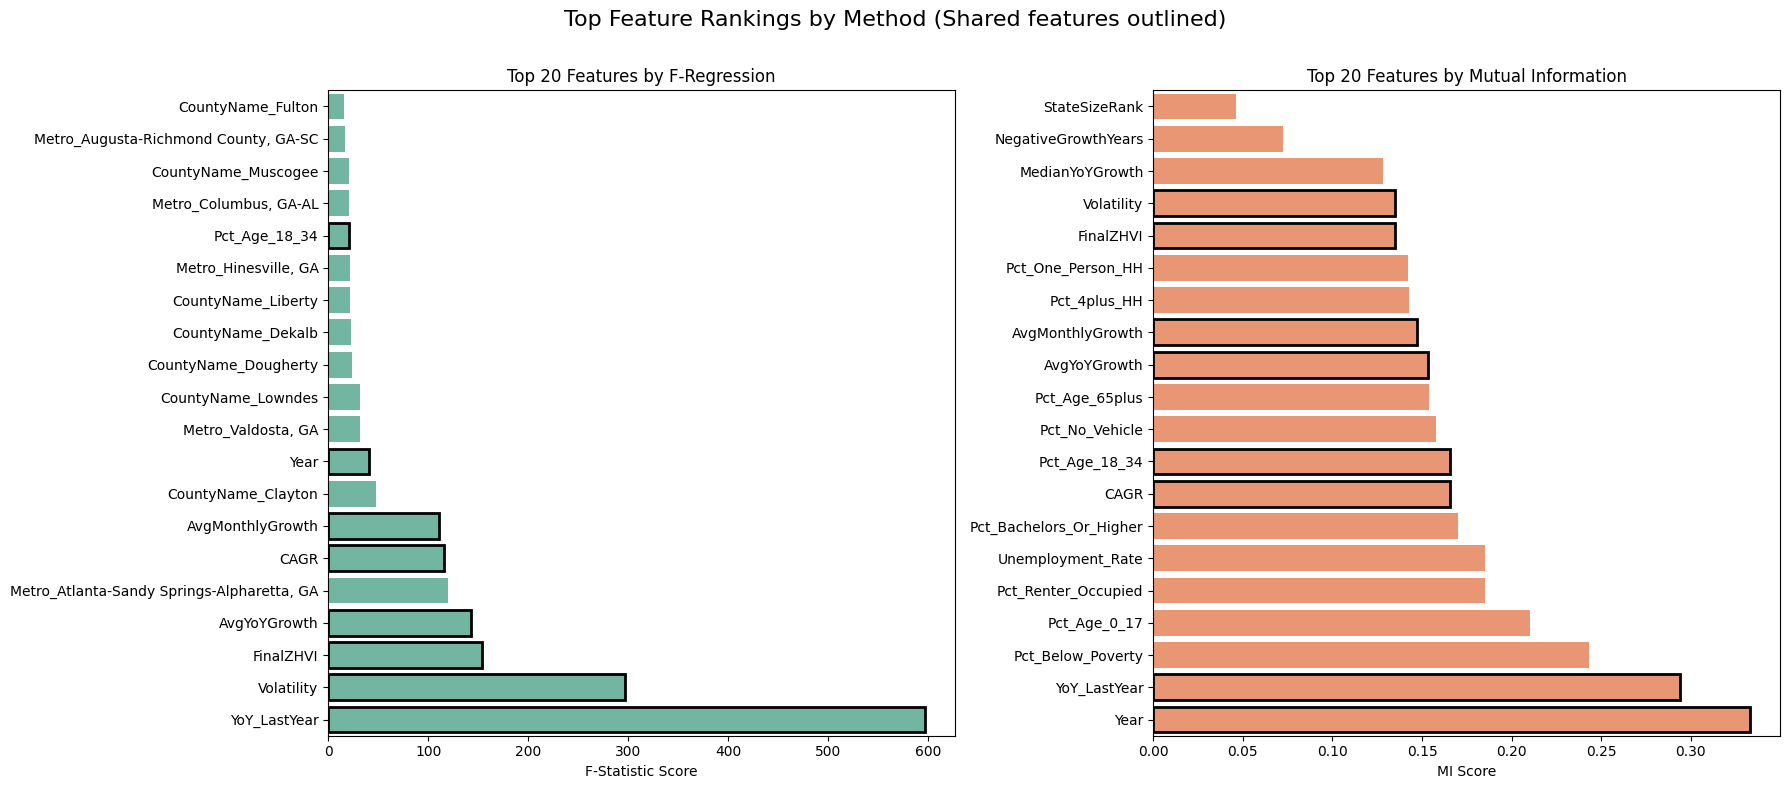
\includegraphics[width=\textwidth]{figures/topfeatures.png}
    \caption{Top 20 features by F-Regression and Mutual Information.}
    \label{fig:top_features}
\end{figure}
\FloatBarrier

Figure~\ref{fig:top_features} shows that features like \texttt{YoY\_LastYear}, \texttt{Volatility}, \texttt{FinalZHVI}, and \texttt{AvgMonthlyGrowth} were among the most informative. Mutual information also highlighted ACS features like poverty and education. These results suggest that both price history and local demographics contribute to future home value trends.

\section{Model training and evaluation}
We tested the following regression models:
\begin{itemize}
    \item Decision Tree,
    \item K-Nearest Neighbors,
    \item Random Forest.
\end{itemize}

Each model was tuned using \texttt{GridSearchCV}. We evaluated performance using:
\begin{itemize}
    \item $R^2$,
    \item RMSE,
    \item MAE,
    \item SMAPE.
\end{itemize}

Performance was reported on the held-out test ZIPs using both metrics and visual inspection of predictions.

\section{Ethical considerations}
The project uses only public datasets with no personal or identifiable information. All data is aggregated at the ZIP or county level. The models are for research and exploration only, and are not meant to support real-world financial decisions.

\section{Summary}
We filtered, cleaned, and reshaped housing data into a rolling ZIP–year format, added engineered time series and ACS features, and carefully split the data by geography to avoid leakage. After ranking features with two methods, we trained and evaluated three models using a consistent pipeline to understand what factors drive next-year home value growth.

    \chapter{Results}
\label{ch:results}

This chapter presents the results of our model training and evaluation. After building and tuning Decision Tree, K-Nearest Neighbors (KNN), and Random Forest regressors using ZIP-based splits, we assessed how well each model predicted year-over-year home value growth. Results are shown across three key areas: model performance with different feature counts, test set prediction accuracy, and model behavior over time for a sample ZIP code.

\section{Feature selection and model comparison}

We first examined how the number of selected features affected each model's performance. For every value of $k$ from 1 to 50, we used both f-regression and mutual information to rank features. The top-$k$ features were then used to compute 3-fold cross-validated $R^2$ scores for each model.

\begin{figure}[!ht]
    \centering
    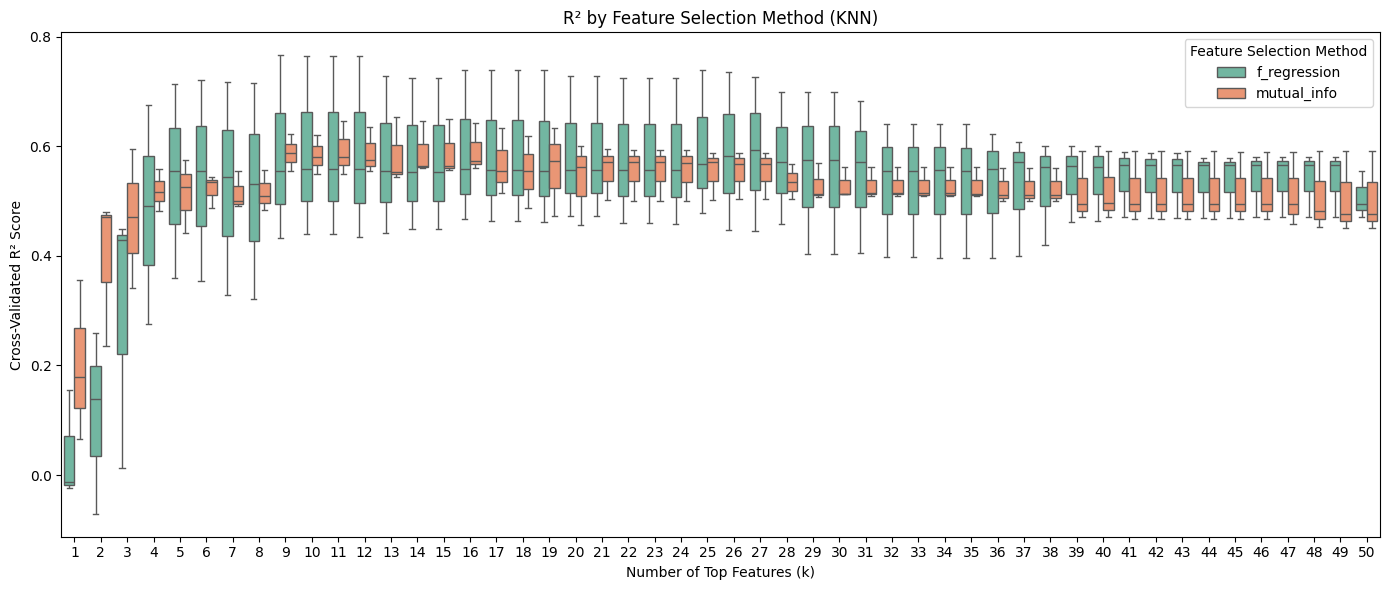
\includegraphics[width=\textwidth]{figures/box50_KNN.png}
    \caption{Cross-validated $R^2$ scores for KNN model.}
    \label{fig:box_knn}
\end{figure}
\FloatBarrier

In Figure~\ref{fig:box_knn}, the KNN model shows a clear performance increase up to about 8 or 9 features, after which the $R^2$ scores plateau. f-regression consistently led to slightly higher performance at low values of $k$, with mutual information catching up as more features were added. Beyond 12–15 features, there was no significant improvement, and some increase in variance was observed, especially with mutual information.

\begin{figure}[!ht]
    \centering
    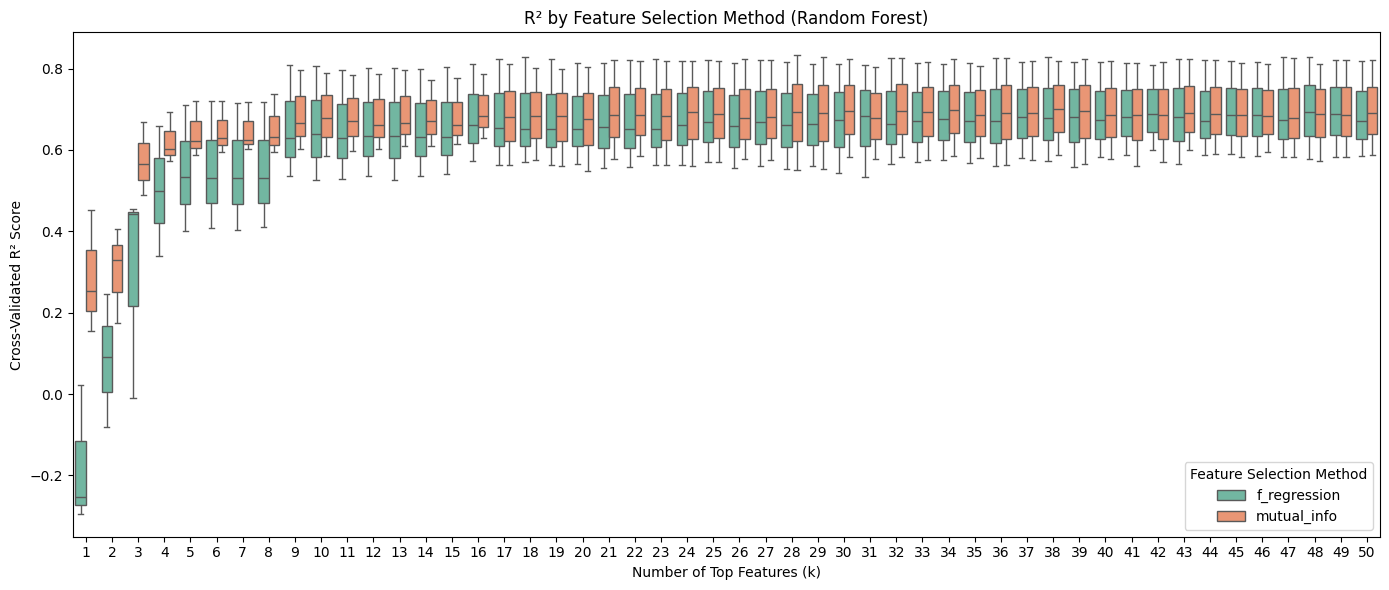
\includegraphics[width=\textwidth]{figures/box50_RF.png}
    \caption{Cross-validated $R^2$ scores for Random Forest model.}
    \label{fig:box_rf}
\end{figure}
\FloatBarrier

Random Forest results in Figure~\ref{fig:box_rf} show a steep improvement in $R^2$ from 1 to around 15 features, peaking between 15–20 features. After that, performance remains mostly stable. The model is more robust to the number of features used, with mutual information providing slightly more consistent results at higher $k$. The box plots are compact throughout, indicating stable behavior across folds.

\begin{figure}[!ht]
    \centering
    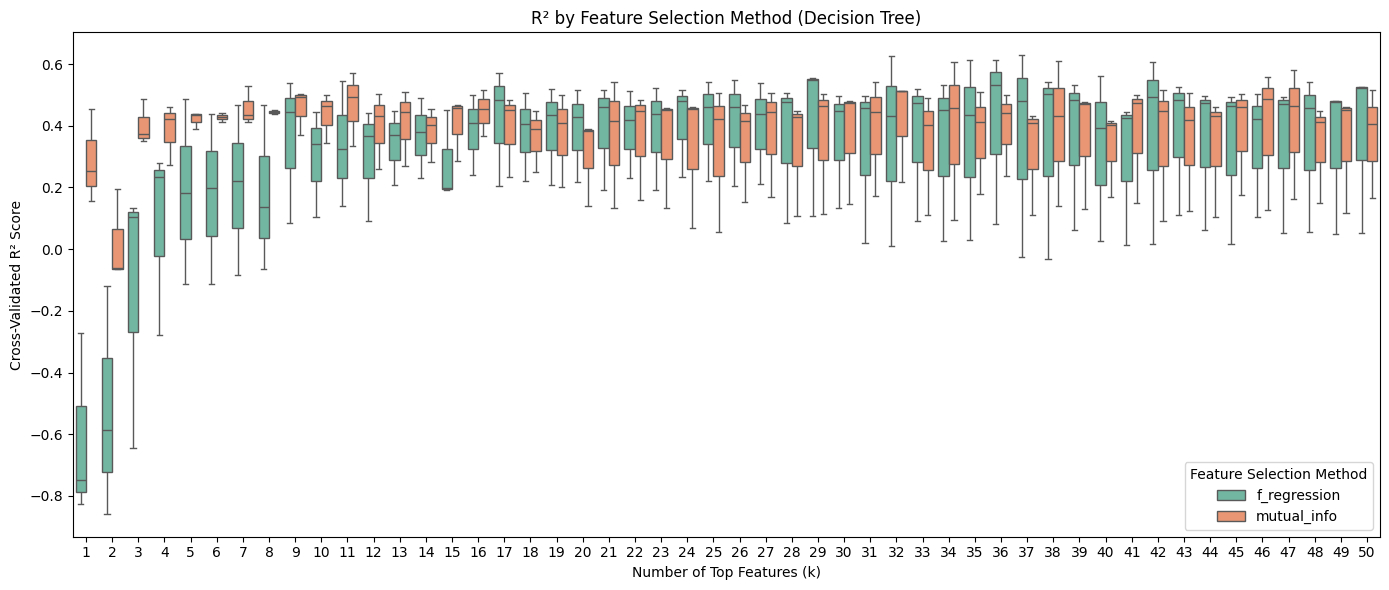
\includegraphics[width=\textwidth]{figures/box50_DT.png}
    \caption{Cross-validated $R^2$ scores for Decision Tree model.}
    \label{fig:box_dt}
\end{figure}
\FloatBarrier

Figure~\ref{fig:box_dt} shows that the Decision Tree model is the most sensitive to the number of features. Performance improves up to around 8–10 features, but quickly deteriorates beyond that, especially with mutual information. This is likely due to overfitting. The most compact and stable results occurred when using 8–12 features, with f-regression performing slightly better overall.

Based on these observations, we selected the following number of features for each model:
\begin{itemize}
    \item \textbf{Decision Tree:} 8 features
    \item \textbf{KNN:} 9 features
    \item \textbf{Random Forest:} 16 features
\end{itemize}

\section{Test set prediction accuracy}

We evaluated each model on a held-out test set of ZIP codes that were not used during training. Figures~\ref{fig:rf_pred}, \ref{fig:knn_pred}, and \ref{fig:dt_pred} show the predicted vs actual year-over-year growth values, along with a regression line, an ideal line ($y = x$), and ±1 RMSE bands.

\begin{figure}[!ht]
    \centering
    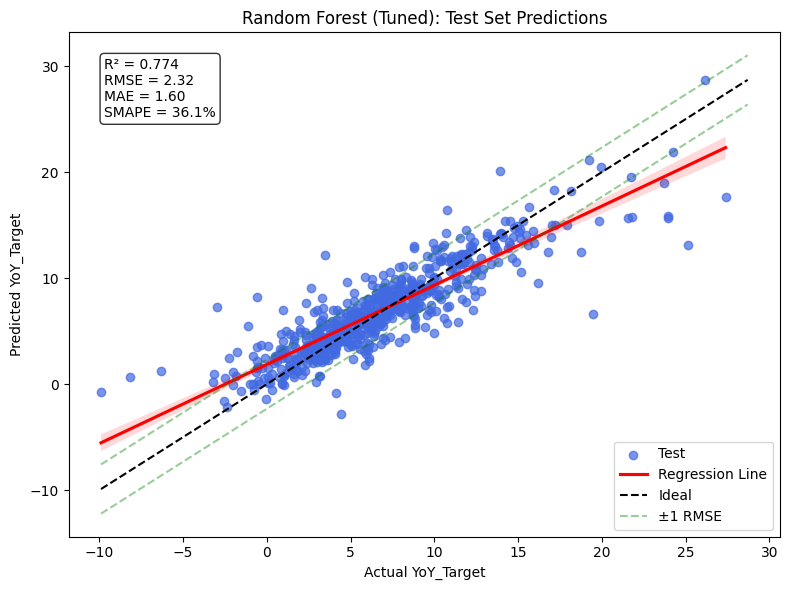
\includegraphics[width=0.75\textwidth]{figures/RF1.png}
    \caption{Random Forest (Tuned): Test set predictions.}
    \label{fig:rf_pred}
\end{figure}
\FloatBarrier

In Figure~\ref{fig:rf_pred}, the Random Forest model shows the strongest test performance. Most predictions fall close to the ideal line, and the regression line closely matches it with a steep slope. The green dashed bands (±1 RMSE) are relatively tight, covering most of the distribution. The model achieved an $R^2$ score of 0.774 on the test set.

\begin{figure}[!ht]
    \centering
    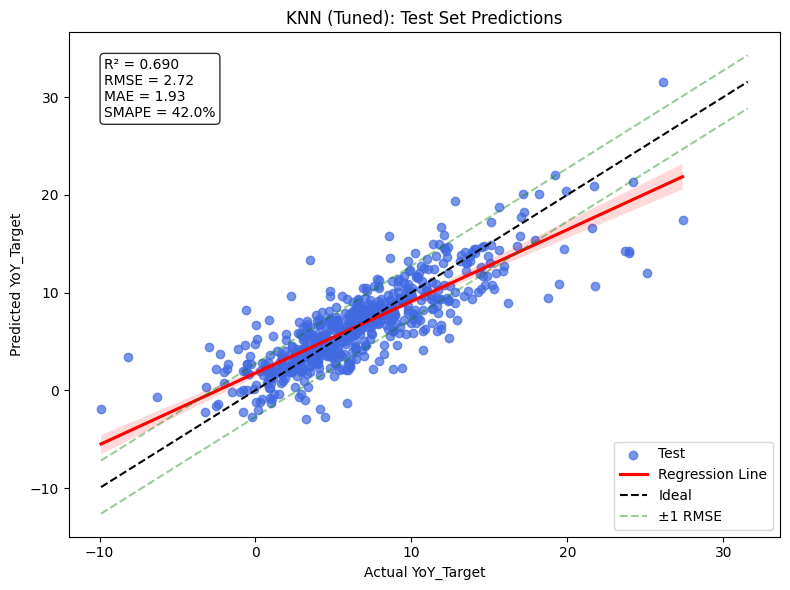
\includegraphics[width=0.75\textwidth]{figures/KNN1.png}
    \caption{KNN (Tuned): Test set predictions.}
    \label{fig:knn_pred}
\end{figure}
\FloatBarrier

The KNN model in Figure~\ref{fig:knn_pred} also performed well, achieving a test $R^2$ of 0.739. Its predictions were slightly more spread out compared to Random Forest, and the regression line was less steep. A few outliers at the higher end of the target range were underpredicted, but the overall alignment to the ideal trend was solid.

\begin{figure}[!ht]
    \centering
    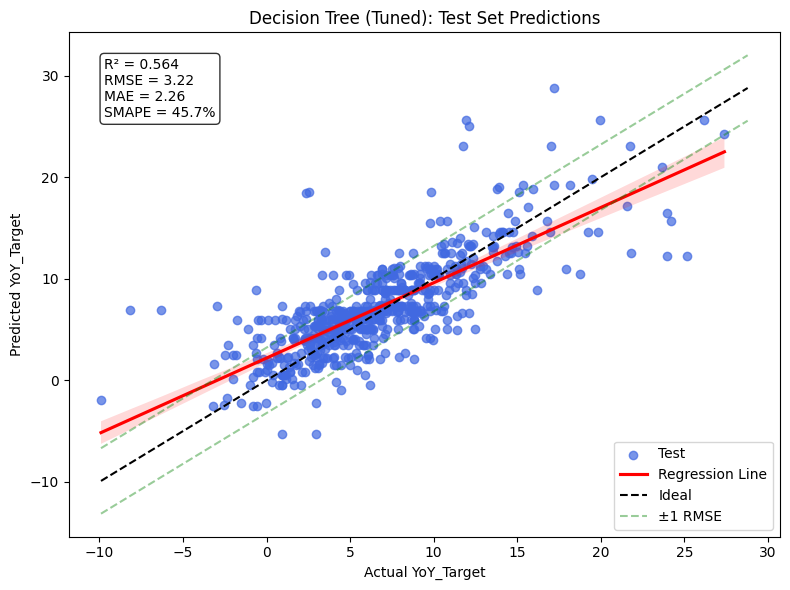
\includegraphics[width=0.75\textwidth]{figures/DT1.png}
    \caption{Decision Tree (Tuned): Test set predictions.}
    \label{fig:dt_pred}
\end{figure}
\FloatBarrier

Figure~\ref{fig:dt_pred} shows the weakest test performance, from the Decision Tree model. Its regression line is noticeably flatter than the ideal, and predictions show more deviation. It underpredicts many higher values and compresses the range of outputs. The test $R^2$ was 0.564, indicating limited generalization.

\section{Train vs test comparison}

To understand how well each model generalizes, we compared train vs test predictions side by side. Figures~\ref{fig:rf_train_test}, \ref{fig:knn_train_test}, and \ref{fig:dt_train_test} show both sets of predictions in one plot.

\begin{figure}[!ht]
    \centering
    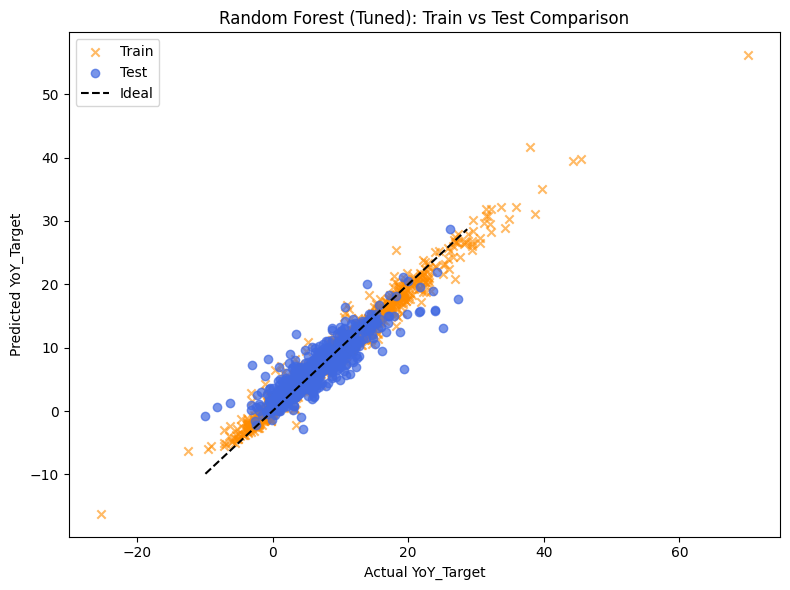
\includegraphics[width=0.75\textwidth]{figures/RF2.png}
    \caption{Random Forest: Train vs test predictions.}
    \label{fig:rf_train_test}
\end{figure}
\FloatBarrier

Figure~\ref{fig:rf_train_test} shows a well-balanced fit for Random Forest. Predictions on both train and test sets are tightly clustered around the ideal line, suggesting the model generalizes well without overfitting.

\begin{figure}[!ht]
    \centering
    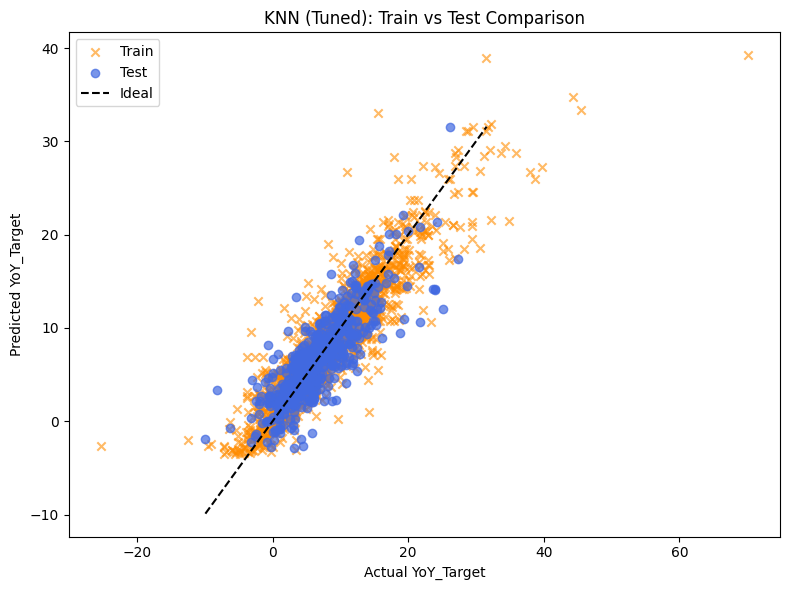
\includegraphics[width=0.75\textwidth]{figures/KNN2.png}
    \caption{KNN: Train vs test predictions.}
    \label{fig:knn_train_test}
\end{figure}
\FloatBarrier

KNN (Figure~\ref{fig:knn_train_test}) also performs consistently across train and test splits, though train predictions are slightly tighter. The test distribution shows slightly more spread, but no major signs of overfitting.

\begin{figure}[!ht]
    \centering
    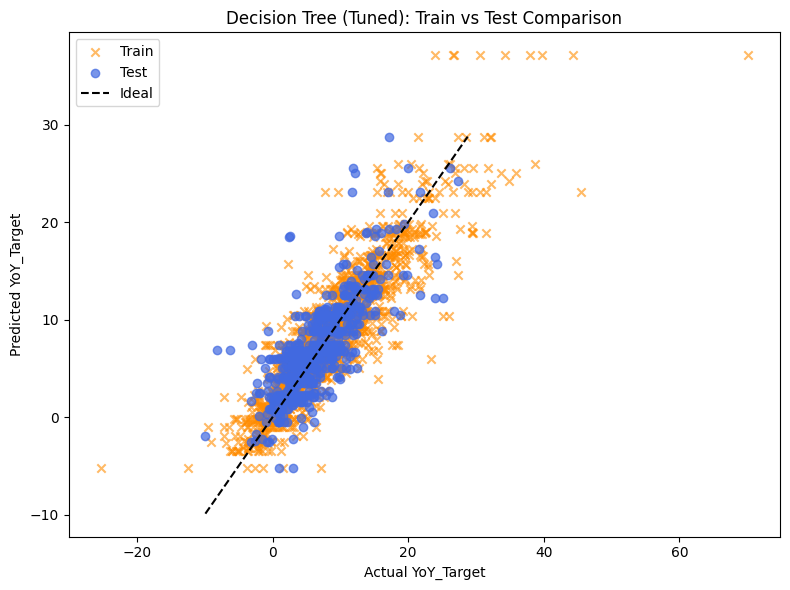
\includegraphics[width=0.75\textwidth]{figures/DT2.png}
    \caption{Decision Tree: Train vs test predictions.}
    \label{fig:dt_train_test}
\end{figure}
\FloatBarrier

The Decision Tree (Figure~\ref{fig:dt_train_test}) shows a stronger fit on the train set than on the test set, with the test predictions exhibiting more variance. This difference suggests some overfitting, consistent with its lower $R^2$ on unseen ZIPs.

\section{Prediction trend over time}

To visualize how each model performs across years for the same location, we selected a ZIP code (31052) and plotted predictions alongside actual YoY values over time.

\begin{figure}[!ht]
    \centering
    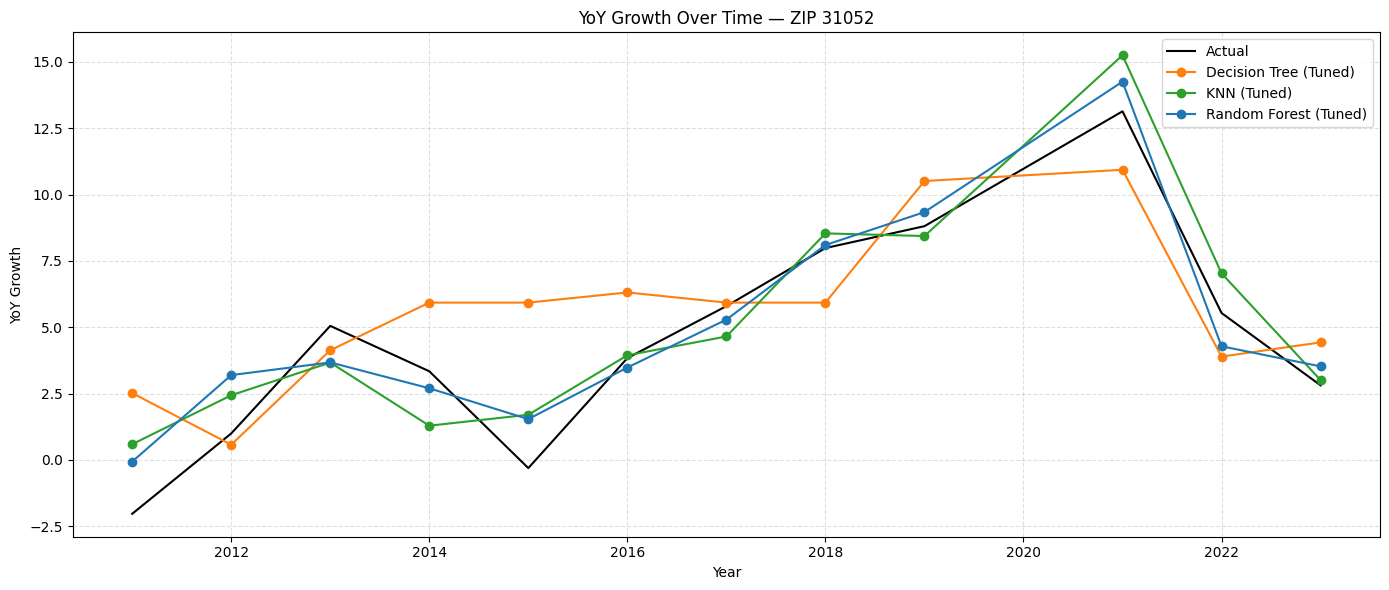
\includegraphics[width=\textwidth]{figures/testpred.png}
    \caption{Predicted vs actual YoY growth over time for ZIP 31052.}
    \label{fig:testpred_zip}
\end{figure}
\FloatBarrier

Figure~\ref{fig:testpred_zip} shows that all models followed the general trend of actual YoY growth, but with different levels of accuracy. Random Forest consistently tracked peaks and dips, while Decision Tree predictions were flatter and missed several changes. KNN captured sharp increases fairly well but overshot in some years. All three models produced usable forecasts, though Random Forest offered the most precise temporal behavior.

\section{Summary of test performance}

Table~\ref{tab:model_results} summarizes final performance on the test set using the selected number of features.

\begin{table}[!ht]
    \centering
    \caption{Model performance on test set (selected features)}
    \label{tab:model_results}
    \begin{tabular}{lcccc}
        \toprule
        \textbf{Model} & \textbf{R\textsuperscript{2}} & \textbf{RMSE} & \textbf{MAE} & \textbf{SMAPE} \\
        \midrule
        Random Forest (16 features) & 0.774 & 2.32 & 1.60 & 36.1\% \\
        KNN (9 features)            & 0.739 & 2.49 & 1.75 & 39.8\% \\
        Decision Tree (8 features) & 0.564 & 3.22 & 2.26 & 45.7\% \\
        \bottomrule
    \end{tabular}
\end{table}
\FloatBarrier

\section{Summary}

All three models captured short-term housing value growth with varying levels of accuracy. Random Forest performed the best across the board, showing strong generalization and tight error margins. KNN followed closely and was relatively stable, but more sensitive to feature selection. Decision Tree required careful tuning and showed signs of overfitting at higher feature counts.

Using both f-regression and mutual information helped ensure that selected features were consistently informative. The ZIP-based split offered a realistic test scenario, ensuring that models were evaluated on truly unseen locations.

    \chapter{Discussion}
\label{ch:discussion}

This chapter discusses why we saw the results we did in the previous section. It focuses on how feature importance was determined, why the models behaved the way they did, and what this tells us about the dataset overall.

\section{Why certain features ranked high}

From both mutual information and f-regression, it was clear that price trend features were the most predictive. Things like previous YoY growth, average monthly growth, volatility, and end-of-year ZHVI consistently ranked at the top. That makes sense, since recent price momentum tends to carry forward, especially in stable markets. These variables give the model a direct view of how each ZIP has been performing recently.

The ACS variables added useful context, especially for areas where price data alone might not be enough. For example, poverty rate, percent with a bachelor's degree or higher, and vehicle ownership were often ranked highly by mutual information. These features probably helped the model adjust for economic conditions that might affect future growth. In particular, education and income levels likely reflect long-term demand and neighborhood stability, even if they're not directly tied to price changes.

f-regression focused more on linear relationships, so it tended to prioritize the ZHVI-based features more heavily. Mutual information captured a broader mix, including nonlinear patterns between demographic indicators and future growth. This explains why mutual information sometimes ranked ACS variables higher, even though they weren't as strong on their own.

\section{Why the models behaved differently}

The Decision Tree performed the worst overall, and the main reason is overfitting. It tried to split on small patterns in the training data that didn’t generalize well. Once we added more than 8–10 features, its performance dropped quickly. This shows that the tree wasn’t able to handle noise or less relevant input. Since it makes hard splits, it doesn’t handle smooth or complex relationships well, especially when features are correlated.

KNN did better, but only up to a point. It works by comparing test ZIPs to similar training ones, so if a ZIP had neighbors in the feature space with similar patterns, it predicted pretty well. But it struggled when a test ZIP didn’t have a close match. It also flattened predictions around the average, which is why it underpredicted at the high end. Adding too many features hurt performance, likely because of the curse of dimensionality. KNN does best with fewer, well-targeted features.

Random Forest was clearly the most stable. It improved as we added more features and didn’t overfit as quickly. That’s expected since it uses many trees with random splits and samples, which helps cancel out noise. It also handles both linear and nonlinear patterns well. Even when some features were weak or redundant, the model still performed consistently. This explains why Random Forest gave us the best test results and tracked the actual growth trends more closely in the time-based plots.

\section{What the prediction patterns tell us}

Looking at the time-based predictions, the models responded differently to trend shifts. Random Forest was the most responsive to real changes — it picked up on dips and rebounds more accurately. That was especially true in volatile years like 2016 or 2023. KNN smoothed over a lot of those changes and generally stayed closer to the mean. Decision Tree sometimes delayed changes or made jumps that didn’t match actual trends.

All models performed better in ZIPs with more stable history. Volatile or sparse ZIPs were harder to predict, and that showed up in the wider spread of test errors. Still, even in those cases, Random Forest was usually closer than the others. It was able to combine short-term trends with economic context to make more reliable predictions.

\section{Limitations to keep in mind}

One limitation is that the ACS data is only available at the county level, so ZIPs within the same county get the same demographic values. This flattens differences between ZIPs that might actually be important. It probably reduced how much impact the ACS variables had in the model. Also, some ZIPs didn’t have enough ZHVI history to calculate good features, so they were excluded entirely.

Another thing to consider is that the target is only one year ahead. While this keeps the setup simple and avoids long-term noise, it also means we’re only capturing short-term effects. A multi-year forecast might show different patterns, especially for slow-changing markets.

\section{Summary}

Overall, the results make sense given the data. The most important predictors were recent price trends and economic indicators that reflect local demand and stability. Random Forest worked best because it could handle complex patterns without overfitting. KNN did well in some cases but was less reliable overall. Decision Tree overfit unless carefully limited. The feature selection helped simplify the models and made it easier to understand what signals were strongest.


    \chapter{Conclusions and Future Work}
\label{ch:con}

\section{Conclusions}

This project explored the feasibility of modeling and predicting year-over-year growth in the Zillow Home Value Index (ZHVI) using historical housing and demographic features at the ZIP code level. The motivation stemmed from the need for data-driven insights to support homebuyers, investors, city planners, and policymakers in understanding local housing market dynamics and identifying high-value growth areas.

A robust pipeline was developed, starting from data collection (Zillow ZHVI and U.S. Census ACS data), followed by preprocessing, feature engineering, model training, and evaluation. Techniques like one-hot encoding, normalization, and feature selection using \texttt{SelectKBest} were critical in handling the complexity and high dimensionality of the data. Models including Decision Tree, K-Nearest Neighbors (KNN), and Random Forest were trained, tuned, and evaluated.

Among these, the \textbf{Random Forest model consistently outperformed} others, highlighting its ability to handle noisy and non-linear housing market data effectively. The ZIP-based data split helped prevent data leakage and ensured the generalizability of the model.

While the model achieved reasonable predictive performance, the limitations in data coverage and geographic scope highlighted areas for future improvement. This project demonstrates that machine learning models, when paired with proper data handling techniques, can serve as valuable tools for interpreting real estate trends and guiding informed decision-making.

\section{Future Work}

\begin{enumerate}
    \item \textbf{Incorporating Material Price Data:} A significant extension would be integrating average material prices into the feature set. This would allow the model to better capture macroeconomic influences on housing costs, offering deeper insight into supply-side drivers of home value changes.

    \item \textbf{Automated Data Updating with AI:} Leveraging AI to automate data ingestion from APIs (such as Zillow, Census, or commodity price feeds) can ensure that the dataset remains up-to-date without manual intervention. This will also allow the model to adapt dynamically as new information becomes available.

    \item \textbf{Multi-Year Growth Modeling:} The current approach focuses on year-over-year changes. Extending this to multi-year trend forecasting would allow stakeholders to plan further into the future and could improve model robustness by capturing long-term dependencies.

    \item \textbf{Improving Temporal and Geographic Flexibility:} Expanding the model to work across broader time periods and more geographic regions can increase its utility. This may involve integrating more granular spatial data or applying transfer learning approaches.

    \item \textbf{Enhanced Visualization and Deployment:} Building a user-facing dashboard that visualizes ZIP code growth predictions and integrates filters for demographics, economic indicators, and material costs could greatly improve accessibility and real-world use.
\end{enumerate}



    

    
    % -------------------------------------------------------------------
    % Bibliography/References  -  Harvard Style was used in this report
    % -------------------------------------------------------------------
    \bibliography{references}  %  Patashnik, O. (1988), BibTEXing. Documentation for general BibTEX users.
    
    % -------------------------------------------------------------------
    % Appendices (if needed)
    % -------------------------------------------------------------------
    
    \begin{appendices}
        \chapter{An Appendix Chapter (Optional)}
\label{appn:A}
% Optional chapter
Some lengthy tables, codes, raw data, length proofs, etc. which are \textbf{very important but not essential part} of the project report goes into an Appendix. An appendix is something a reader would consult if he/she needs extra information and a more comprehensive understating of the report. Also, note that you should use one appendix for one idea.

An appendix is optional. If you feel you do not need to include an appendix in your report, avoid including it. Sometime including irrelevant and unnecessary materials in the Appendices may unreasonably increase the total number of pages in your report and distract the reader.


        \chapter{An Appendix Chapter (Optional)}
\label{appn:B}

...
    \end{appendices}
    
\end{document}
